\documentclass{article}
\usepackage{graphicx}
\usepackage{listings}
\usepackage[strings]{underscore}

\begin{document}
\section{Time for CPU Conversion}
\begin{lstlisting}[language=Python]
height = img.shape[0]
width = img.shape[1]

cpu_gray_image = [
    [0 for _ in range(width)]
    for _ in range(height)
]

start = time.time()

for y in range(height):
    for x in range(width):
        r = int(img[y, x, 0])
        g = int(img[y, x, 1])
        b = int(img[y, x, 2])
        gray = (r + g + b) // 3
        cpu_gray_image[y][x] = gray

end = time.time()

print(f"CPU time: {end - start:.6f} seconds")
\end{lstlisting}
\begin{verbatim}
-> Results: CPU time: 0.266899 seconds
\end{verbatim}

\section{Time for GPU Conversion}
\begin{lstlisting}[language=Python]
@cuda.jit
def grayscale_kernel(input_img, output_img):
    tidx = cuda.threadIdx.x + cuda.blockIdx.x * cuda.blockDim.x
    g = np.uint8((input_img[tidx, 0] + input_img[tidx, 1] + input_img[tidx, 2]) / 3)
    output_img[tidx, 0] = output_img[tidx, 1] = output_img[tidx, 2] = g

original_shape = img.shape
img_flat = img.reshape(-1, 3).astype(np.uint8)

d_img = cuda.to_device(img_flat)
d_grayscale_img = cuda.device_array(
    img_flat.shape,
    dtype=np.uint8
)
pixelCount = img_flat.shape[0]
blockSize = 256
gridSize = (pixelCount + blockSize - 1) // blockSize
start = time.time()
grayscale_kernel[gridSize, blockSize](d_img, d_grayscale_img)
cuda.synchronize()
end = time.time()
grayscale_img = d_grayscale_img.copy_to_host()
print(f"GPU time: {end - start:.6f} seconds")
\end{lstlisting}
\begin{verbatim}
Explaination: 
1st: Flatten the image and send it to gpu
2nd: Create a device array to store the result
3rd: Calculate the grid size and block size
4th: Call the kernel function and synchronize
5th: Copy the result back to host and reshape it to original shape
-> Results: GPU time: 0.056622 seconds
\end{verbatim}

\section{Block size vs Time}
\begin{figure}[htbp]
    \centering
    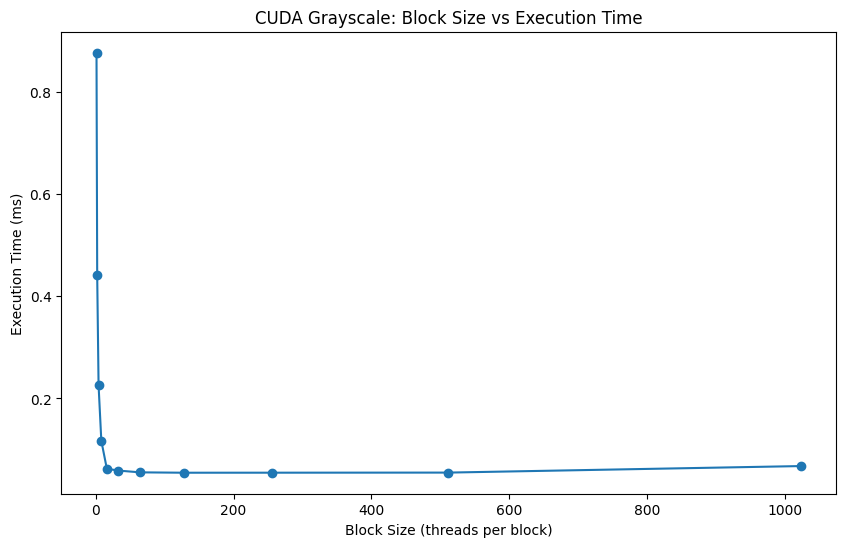
\includegraphics[width=0.85\textwidth]{block_size_vs_time.png}
    \caption{Block size vs Time}
\end{figure}
- Increase the block size, the time will decrease. The optimal block size is 256.
\end{document}
